\documentclass[11pt]{report}

% Paquetes y configuraciones adicionales
\usepackage{graphicx}
\usepackage[export]{adjustbox}
\usepackage{caption}
\usepackage{float}
\usepackage{titlesec}
\usepackage{geometry}
\usepackage[hidelinks]{hyperref}
\usepackage{titling}
\usepackage{titlesec}
\usepackage{parskip}
\usepackage{wasysym}
\usepackage{tikzsymbols}
\usepackage{fancyvrb}
\usepackage{xurl}
\usepackage{hyperref}
\usepackage[spanish]{babel}

\newcommand{\subtitle}[1]{
  \posttitle{
    \par\end{center}
    \begin{center}\large#1\end{center}
    \vskip0.5em}
}

% Configura los márgenes
\geometry{
  left=2cm,   % Ajusta este valor al margen izquierdo deseado
  right=2cm,  % Ajusta este valor al margen derecho deseado
  top=3cm,
  bottom=3cm,
}

% Configuración de los títulos de las secciones
\titlespacing{\section}{0pt}{\parskip}{\parskip}
\titlespacing{\subsection}{0pt}{\parskip}{\parskip}
\titlespacing{\subsubsection}{0pt}{\parskip}{\parskip}

% Redefinir el formato de los capítulos y añadir un punto después del número
\makeatletter
\renewcommand{\@makechapterhead}[1]{%
  \vspace*{0\p@} % Ajusta este valor para el espaciado deseado antes del título del capítulo
  {\parindent \z@ \raggedright \normalfont
    \ifnum \c@secnumdepth >\m@ne
        \huge\bfseries \thechapter.\ % Añade un punto después del número
    \fi
    \interlinepenalty\@M
    #1\par\nobreak
    \vspace{10pt} % Ajusta este valor para el espacio deseado después del título del capítulo
  }}
\makeatother

% Configura para que cada \chapter no comience en una pagina nueva
\makeatletter
\renewcommand\chapter{\@startsection{chapter}{0}{\z@}%
    {-3.5ex \@plus -1ex \@minus -.2ex}%
    {2.3ex \@plus.2ex}%
    {\normalfont\Large\bfseries}}
\makeatother

%==============================================================================
% Cosas para la documentación LateX
% % Sangría
% \setlength{\parindent}{1em}Texto

% % Quitar sangría
% \noindent

% % Punto
% \CIRCLE \ \ \textbf{Texto} \emph{algo}
% \begin{itemize}
%   \item \textbf{Negrita:} Texto
%   \item \textbf{Negrita:} Texto
% \end{itemize}

% % Introducir código
% \begin{center}
%   \begin{BVerbatim}
%     ... Código
%   \end{BVerbatim}
% \end{center}

% Poner una imagen
% \begin{figure}[H]
%   \centering
%   \includegraphics[scale=0.55]{img/}
%   \caption{Exportación de la base de datos en formato sql}
%   \label{fig:exportación de la base de datos en formato sql}
% \end{figure}

% % Poner una tabla
% \begin{table}[H]
%   \centering
%   \begin{tabular}{|c|c|c|c|}
%     \hline
%     \textbf{Campo 1} & \textbf{Campo 2} & \textbf{Campo 3} & \textbf{Campo 4} \\ \hline
%     Texto & Texto & Texto & Texto \\ \hline
%     Texto & Texto & Texto & Texto \\ \hline
%     Texto & Texto & Texto & Texto \\ \hline
%     Texto & Texto & Texto & Texto \\ \hline
%   \end{tabular}
%   \caption{Nombre de la tabla}
%   \label{tab:nombre de la tabla}
% \end{table}

%==============================================================================

\begin{document}

% Portada del informe
\title{Práctica 05. Índices y optimizacion de las bases de datos}
\subtitle{Adminstración y Diseño de Bases de Datos}
\author{Cheuk Kelly Ng Pante (alu0101364544@ull.edu.es)}
\date{29 de noviembre de 2023}

\maketitle

\pagestyle{empty} % Desactiva la numeración de página para el índice

% Índice
\tableofcontents

% Nueva página
\cleardoublepage

\pagestyle{plain} % Vuelve a activar la numeración de página
\setcounter{page}{1} % Reinicia el contador de página a 1

% Secciones del informe
% Capitulo 1
\chapter{Restauracion de la base de datos \emph{postgres\_air}}
Para la restauración de la base de datos se ha optado por usar la base de datos \emph{postgres\_air.backup}.
Antes de restaurar la base de datos, hay que crear la base de datos \emph{postgres\_air}, primero entramos
en la consola de postgres y luego creamos la base de datos con la siguiente sentencia:
\begin{center}
  \begin{BVerbatim}
    CREATE DATABASE postgres_air;
  \end{BVerbatim}
\end{center}

Una vez creada la base de datos, la restauramos con el siguiente comando:
\begin{center}
  \begin{BVerbatim}
    pg_restore -x --no-owner -U postgres -d postgres_air ./postgres_air.backup
  \end{BVerbatim}
\end{center}

% Capitulo 2
\chapter{Incluir sentencias SQL para la creación de los índices}
Tenemos las siguientes sentencias SQL:
\begin{figure}[H]
  \centering
  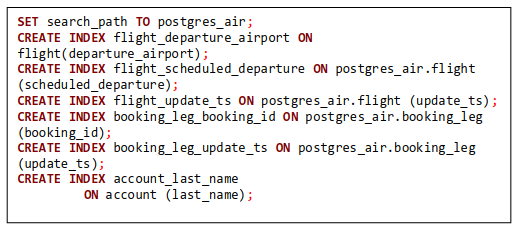
\includegraphics[scale=0.65]{img/sentencias_sql.png}
  \caption{Sentencias SQL}
  \label{fig:sentencias SQL}
\end{figure}

Lo que hacen estas sentencias es crear índices en las tablas y atributos más consultados. De estas
manera el rendimiento de la base de datos mejora sustancialmente. 

Aqui una captura de pantalla de la ejecución de las sentencias SQL:
\begin{figure}[H]
  \centering
  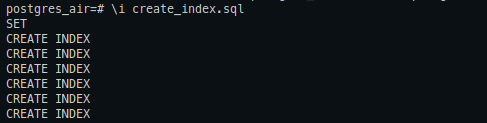
\includegraphics[scale=0.65]{img/ejecucion_create_index.png}
  \caption{Ejecución de las sentencias SQL}
  \label{fig:ejecución de las sentencias SQL}
\end{figure}

% Nueva página
\cleardoublepage

% Capitulo 3
\chapter{Identifique las tablas principales y sus principales elementos}
Las tablas principales son las siguientes:
\begin{itemize}
  \item \textbf{accounts:} Contiene información de las cuentas de los usuarios.
    \subitem \textbf{account\_id:} Identificador de la cuenta, de tipo \emph{INTEGER}.
    \subitem \textbf{login:} Nombre de usuario, de tipo \emph{TEXT}.
    \subitem \textbf{first\_name} Nombre del usuario, de tipo \emph{TEXT}.
    \subitem \textbf{last\_name} Apellido del usuario, de tipo \emph{TEXT}.
    \subitem \textbf{frequent\_flyer\_id} Identificador del viajero frecuente, de tipo \emph{INTEGER}.
    \subitem \textbf{update\_ts} Fecha de actualización, de tipo \emph{TIMESTAMP WITH TIME ZONE}.
  \item \textbf{aircraft:} Contiene información de los aviones.
    \subitem \textbf{model} Modelo del avión, de tipo \emph{TEXT}.
    \subitem \textbf{range} Rango del avión, de tipo \emph{NUMERIC}.
    \subitem \textbf{class} Clase del avión, de tipo \emph{INTEGER}.
    \subitem \textbf{velocity} Velocidad del avión, de tipo \emph{NUMERIC}.
    \subitem \textbf{code} Código del avión, de tipo \emph{TEXT}.
  \item \textbf{airport:} Contiene información de los aeropuertos.
    \subitem \textbf{airport\_code} Código del aeropuerto, de tipo \emph{CHARACTER(3)}.
    \subitem \textbf{airport\_name} Nombre del aeropuerto, de tipo \emph{TEXT}.
    \subitem \textbf{city} Ciudad del aeropuerto, de tipo \emph{TEXT}.
    \subitem \textbf{airport\_tz} Zona horaria del aeropuerto, de tipo \emph{TEXT}.
    \subitem \textbf{continent} Continente del aeropuerto, de tipo \emph{TEXT}.
    \subitem \textbf{iso\_country} Código del país del aeropuerto, de tipo \emph{TEXT}.
    \subitem \textbf{iso\_region} Código de la región del aeropuerto, de tipo \emph{TEXT}.
    \subitem \textbf{intnl} Si el aeropuerto es internacional o no, de tipo \emph{BOOLEAN}.
    \subitem \textbf{update\_ts} Fecha de actualización, de tipo \emph{TIMESTAMP WITH TIME ZONE}.
  \item \textbf{boarding\_pass:} Contiene información de las tarjetas de embarque.
    \subitem \textbf{pass\_id} Identificador de la tarjeta de embarque, de tipo \emph{INTEGER}.
    \subitem \textbf{passenger\_id} Identificador del pasajero, de tipo \emph{BIGINT}.
    \subitem \textbf{booking\_leg\_id} Identificador de la reserva del vuelo, de tipo \emph{BIGINT}.
    \subitem \textbf{seat} Asiento del pasajero, de tipo \emph{TEXT}.
    \subitem \textbf{boarding\_time} Fecha de embarque, de tipo \emph{TIMESTAMP WITH TIME ZONE}.
    \subitem \textbf{precheck} Si el pasajero ha hecho el check-in o no, de tipo \emph{BOOLEAN}.
    \subitem \textbf{update\_ts} Fecha de actualización, de tipo \emph{TIMESTAMP WITH TIME ZONE}.
  \item \textbf{booking:} Contiene información de las reservas.
    \subitem \textbf{booking\_id} Identificador de la reserva, de tipo \emph{BIGINT}.
    \subitem \textbf{booking\_ref} Referencia de la reserva, de tipo \emph{TEXT}.
    \subitem \textbf{booking\_name} Nombre de la reserva, de tipo \emph{TEXT}.
    \subitem \textbf{account\_id} Identificador de la cuenta, de tipo \emph{INTEGER}.
    \subitem \textbf{email} Correo electrónico, de tipo \emph{TEXT}.
    \subitem \textbf{phone} Teléfono, de tipo \emph{TEXT}.
    \subitem \textbf{update\_ts} Fecha de actualización, de tipo \emph{TIMESTAMP WITH TIME ZONE}.
    \subitem \textbf{price} Precio de la reserva, de tipo \emph{NUMERIC}.
  \item \textbf{booking\_leg:} Contiene información de las reservas de los vuelos.
    \subitem \textbf{booking\_leg\_id} Identificador de la reserva del vuelo, de tipo \emph{INTEGER}.
    \subitem \textbf{booking\_id} Identificador de la reserva, de tipo \emph{INTEGER}.
    \subitem \textbf{flight\_id} Identificador del vuelo, de tipo \emph{INTEGER}.
    \subitem \textbf{leg\_num} Número de la reserva del vuelo, de tipo \emph{INTEGER}.
    \subitem \textbf{is\_returning} Si el vuelo es de vuelta o no, de tipo \emph{BOOLEAN}.
    \subitem \textbf{update\_ts} Fecha de actualización, de tipo \emph{TIMESTAMP WITH TIME ZONE}.
  \item \textbf{flight:} Contiene información de los vuelos.
    \subitem \textbf{flight\_id} Identificador del vuelo, de tipo \emph{INTEGER}.
    \subitem \textbf{flight\_no} Número del vuelo, de tipo \emph{TEXT}.
    \subitem \textbf{scheduled\_departure} Fecha de salida programada, tipo \emph{TIMESTAMP WITH TIME ZONE}.
    \subitem \textbf{scheduled\_arrival} Fecha de llegada programada, de tipo \emph{TIMESTAMP WITH TIME ZONE}.
    \subitem \textbf{departure\_airport} Código del aeropuerto de salida, de tipo \emph{CHARACTER(3)}.
    \subitem \textbf{arrival\_airport} Código del aeropuerto de llegada, de tipo \emph{CHARACTER(3)}.
    \subitem \textbf{status} Estado del vuelo, de tipo \emph{TEXT}.
    \subitem \textbf{aircraft\_code} Código del avión, de tipo \emph{CHARACTER(3)}.
    \subitem \textbf{actual\_departure} Fecha de salida actual, de tipo \emph{TIMESTAMP WITH TIME ZONE}.
    \subitem \textbf{actual\_arrival} Fecha de llegada actual, de tipo \emph{TIMESTAMP WITH TIME ZONE}.
    \subitem \textbf{update\_ts} Fecha de actualización, de tipo \emph{TIMESTAMP WITH TIME ZONE}.
  \item \textbf{frequent\_flyer:} Contiene información de los viajeros frecuentes.
    \subitem \textbf{frequent\_flyer\_id} Identificador del viajero frecuente, de tipo \emph{INTEGER}.
    \subitem \textbf{first\_name} Nombre del viajero frecuente, de tipo \emph{TEXT}.
    \subitem \textbf{last\_name} Apellido del viajero frecuente, de tipo \emph{TEXT}.
    \subitem \textbf{title} Título del viajero frecuente, de tipo \emph{TEXT}.
    \subitem \textbf{card\_num} Número de la tarjeta del viajero frecuente, de tipo \emph{TEXT}.
    \subitem \textbf{level} Nivel del viajero frecuente, de tipo \emph{INTEGER}.
    \subitem \textbf{award\_points} Puntos del viajero frecuente, de tipo \emph{INTEGER}.
    \subitem \textbf{email} Correo electrónico del viajero frecuente, de tipo \emph{TEXT}.
    \subitem \textbf{phone} Teléfono del viajero frecuente, de tipo \emph{TEXT}.
    \subitem \textbf{update\_ts} Fecha de actualización, de tipo \emph{TIMESTAMP WITH TIME ZONE}.
  \item \textbf{passenger:} Contiene información de los pasajeros.
    \subitem \textbf{passenger\_id} Identificador del pasajero, de tipo \emph{INTEGER}.
    \subitem \textbf{booking\_id} Identificador de la reserva, de tipo \emph{INTEGER}.
    \subitem \textbf{booking\_ref} Referencia de la reserva, de tipo \emph{TEXT}.
    \subitem \textbf{passenger\_no} Número del pasajero, de tipo \emph{INTEGER}.
    \subitem \textbf{first\_name} Nombre del pasajero, de tipo \emph{TEXT}.
    \subitem \textbf{last\_name} Apellido del pasajero, de tipo \emph{TEXT}.
    \subitem \textbf{account\_id} Identificador de la cuenta, de tipo \emph{INTEGER}.
    \subitem \textbf{update\_ts} Fecha de actualización, de tipo \emph{TIMESTAMP WITH TIME ZONE}.
    \subitem \textbf{age} Edad del pasajero, de tipo \emph{INTEGER}.
  \item \textbf{phone:} Contiene información de los teléfonos.
    \subitem \textbf{phone\_id} Identificador del teléfono, de tipo \emph{INTEGER}.
    \subitem \textbf{account\_id} Identificador de la cuenta, de tipo \emph{INTEGER}.
    \subitem \textbf{phone} Teléfono, de tipo \emph{TEXT}.
    \subitem \textbf{phone\_type} Tipo de teléfono, de tipo \emph{TEXT}.
    \subitem \textbf{primary\_phone} Si es el teléfono principal o no, de tipo \emph{BOOLEAN}.
    \subitem \textbf{update\_ts} Fecha de actualización, de tipo \emph{TIMESTAMP WITH TIME ZONE}.
\end{itemize}

% Nueva página
\cleardoublepage

% Capitulo 4
\chapter{Diagrama Entidad-Relación}
% \begin{figure}[H]
%   \centering
%   \includegraphics[scale=0.65]{img/diagrama_entidad_relacion.png}
%   \caption{Diagrama Entidad-Relación}
%   \label{fig:diagrama Entidad-Relación}
% \end{figure}

% Nueva página
\cleardoublepage

% Capitulo 5
\chapter{Realizar la siguiente consulta}
\begin{figure}[H]
  \centering
  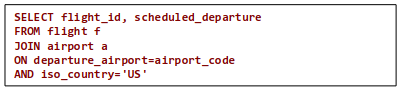
\includegraphics[scale=0.75]{img/consulta_5.png}
  \label{fig:consulta}
\end{figure}

\section{Utilizar \emph{EXPLAIN} para obtener el plan de consulta}
\begin{figure}[H]
  \centering
  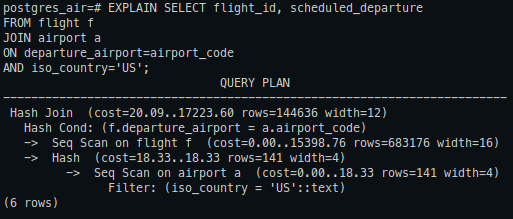
\includegraphics[scale=0.6]{img/consulta_explain.png}
  \caption{Consulta con \emph{EXPLAIN}}
  \label{fig:consulta con EXPLAIN}
\end{figure}

\section{Obtener información de la consulta \emph{EXPLAIN}}
\begin{itemize}
  \item \textbf{Costo total de la consulta:} 17223.60 unidades.
  \item \textbf{Costo de configuración:}  20.09 unidades.
  \item \textbf{Cantidad de filas que se devolverán:} 144636 filas.
  \item \textbf{Cantidad de filas estimadas:} 683176 filas.
\end{itemize}

\section{Repetir la consulta con \emph{EXPLAIN} con un limite de 15 registros}
\begin{figure}[H]
  \centering
  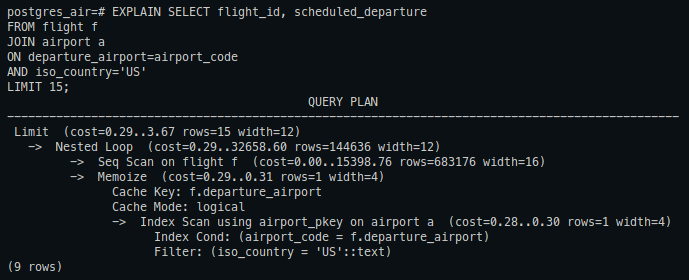
\includegraphics[scale=0.55]{img/consulta_explain_limit.png}
  \caption{Consulta con \emph{EXPLAIN} y límite de 15 registros}
  \label{fig:consulta con EXPLAIN y límite de 15 registros}
\end{figure}

% postgres_air=# EXPLAIN SELECT flight_id, scheduled_departure
% FROM flight f
% JOIN airport a
% ON departure_airport=airport_code
% AND iso_country='US'
% LIMIT 15;
%                                            QUERY PLAN                                           
% ------------------------------------------------------------------------------------------------
%  Limit  (cost=0.29..3.67 rows=15 width=12)
%    ->  Nested Loop  (cost=0.29..32658.60 rows=144636 width=12)
%          ->  Seq Scan on flight f  (cost=0.00..15398.76 rows=683176 width=16)
%          ->  Memoize  (cost=0.29..0.31 rows=1 width=4)
%                Cache Key: f.departure_airport
%                Cache Mode: logical
%                ->  Index Scan using airport_pkey on airport a  (cost=0.28..0.30 rows=1 width=4)
%                      Index Cond: (airport_code = f.departure_airport)
%                      Filter: (iso_country = 'US'::text)
% (9 rows)

\section{Obtener información de la consulta \emph{EXPLAIN} con un limite de 15 registros}
Hay una reducción del costo abismal. Hay en total 2 pasos principales, que son dos los
dos Merges. El segundo de esto se subdivide en otros dos en donde consulta los índices
previamente creados.

\begin{itemize}
  \item \textbf{Costo del paso limitante:} 3.67 unidades.
  \item \textbf{Costo de configuración:}  0.29 unidades.
  \item \textbf{Cantidad de filas que se devolverán:} 15 filas.
  \item \textbf{Cantidad de filas estimadas:} 144636 filas.
\end{itemize}

% Nueva página
\cleardoublepage

% Capitulo 6
\chapter{Realizar la siguiente consulta similar a la anterior}

% Nueva página
\cleardoublepage

\chapter{Bibliografía} % En formato APA
\begin{enumerate}
\item Ng Pante, C. (2001). Titulo. Nombre pagina web. Recuperado de \url{http://url.com}

\end{enumerate}

\end{document}